\documentclass[11pt]{IEEEtran}
\usepackage{graphicx}
\usepackage{url}

\ifCLASSINFOpdf
  % \usepackage[pdftex]{graphicx}
  % declare the path(s) where your graphic files are
  % \graphicspath{{../pdf/}{../jpeg/}}
  % and their extensions so you won't have to specify these with
  % every instance of \includegraphics
  % \DeclareGraphicsExtensions{.pdf,.jpeg,.png}
\else
  % or other class option (dvipsone, dvipdf, if not using dvips). graphicx
  % will default to the driver specified in the system graphics.cfg if no
  % driver is specified.
  % \usepackage[dvips]{graphicx}
  % declare the path(s) where your graphic files are
  % \graphicspath{{../eps/}}
  % and their extensions so you won't have to specify these with
  % every instance of \includegraphics
  % \DeclareGraphicsExtensions{.eps}
\fi
% graphicx was written by David Carlisle and Sebastian Rahtz. It is
% required if you want graphics, photos, etc. graphicx.sty is already
% installed on most LaTeX systems. The latest version and documentation can
% be obtained at: 
% http://www.ctan.org/tex-archive/macros/latex/required/graphics/
% Another good source of documentation is "Using Imported Graphics in
% LaTeX2e" by Keith Reckdahl which can be found as epslatex.ps or
% epslatex.pdf at: http://www.ctan.org/tex-archive/info/
%
% latex, and pdflatex in dvi mode, support graphics in encapsulated
% postscript (.eps) format. pdflatex in pdf mode supports graphics
% in .pdf, .jpeg, .png and .mps (metapost) formats. Users should ensure
% that all non-photo figures use a vector format (.eps, .pdf, .mps) and
% not a bitmapped formats (.jpeg, .png). IEEE frowns on bitmapped formats
% which can result in "jaggedy"/blurry rendering of lines and letters as
% well as large increases in file sizes.
%
% You can find documentation about the pdfTeX application at:
% http://www.tug.org/applications/pdftex





% *** MATH PACKAGES ***
%
%\usepackage[cmex10]{amsmath}
% A popular package from the American Mathematical Society that provides
% many useful and powerful commands for dealing with mathematics. If using
% it, be sure to load this package with the cmex10 option to ensure that
% only type 1 fonts will utilized at all point sizes. Without this option,
% it is possible that some math symbols, particularly those within
% footnotes, will be rendered in bitmap form which will result in a
% document that can not be IEEE Xplore compliant!
%
% Also, note that the amsmath package sets \interdisplaylinepenalty to 10000
% thus preventing page breaks from occurring within multiline equations. Use:
%\interdisplaylinepenalty=2500
% after loading amsmath to restore such page breaks as IEEEtran.cls normally
% does. amsmath.sty is already installed on most LaTeX systems. The latest
% version and documentation can be obtained at:
% http://www.ctan.org/tex-archive/macros/latex/required/amslatex/math/





% *** SPECIALIZED LIST PACKAGES ***
%
%\usepackage{algorithmic}
% algorithmic.sty was written by Peter Williams and Rogerio Brito.
% This package provides an algorithmic environment fo describing algorithms.
% You can use the algorithmic environment in-text or within a figure
% environment to provide for a floating algorithm. Do NOT use the algorithm
% floating environment provided by algorithm.sty (by the same authors) or
% algorithm2e.sty (by Christophe Fiorio) as IEEE does not use dedicated
% algorithm float types and packages that provide these will not provide
% correct IEEE style captions. The latest version and documentation of
% algorithmic.sty can be obtained at:
% http://www.ctan.org/tex-archive/macros/latex/contrib/algorithms/
% There is also a support site at:
% http://algorithms.berlios.de/index.html
% Also of interest may be the (relatively newer and more customizable)
% algorithmicx.sty package by Szasz Janos:
% http://www.ctan.org/tex-archive/macros/latex/contrib/algorithmicx/




% *** ALIGNMENT PACKAGES ***
%
%\usepackage{array}
% Frank Mittelbach's and David Carlisle's array.sty patches and improves
% the standard LaTeX2e array and tabular environments to provide better
% appearance and additional user controls. As the default LaTeX2e table
% generation code is lacking to the point of almost being broken with
% respect to the quality of the end results, all users are strongly
% advised to use an enhanced (at the very least that provided by array.sty)
% set of table tools. array.sty is already installed on most systems. The
% latest version and documentation can be obtained at:
% http://www.ctan.org/tex-archive/macros/latex/required/tools/


%\usepackage{mdwmath}
%\usepackage{mdwtab}
% Also highly recommended is Mark Wooding's extremely powerful MDW tools,
% especially mdwmath.sty and mdwtab.sty which are used to format equations
% and tables, respectively. The MDWtools set is already installed on most
% LaTeX systems. The lastest version and documentation is available at:
% http://www.ctan.org/tex-archive/macros/latex/contrib/mdwtools/


% IEEEtran contains the IEEEeqnarray family of commands that can be used to
% generate multiline equations as well as matrices, tables, etc., of high
% quality.


%\usepackage{eqparbox}
% Also of notable interest is Scott Pakin's eqparbox package for creating
% (automatically sized) equal width boxes - aka "natural width parboxes".
% Available at:
% http://www.ctan.org/tex-archive/macros/latex/contrib/eqparbox/





% *** SUBFIGURE PACKAGES ***
%\usepackage[tight,footnotesize]{subfigure}
% subfigure.sty was written by Steven Douglas Cochran. This package makes it
% easy to put subfigures in your figures. e.g., "Figure 1a and 1b". For IEEE
% work, it is a good idea to load it with the tight package option to reduce
% the amount of white space around the subfigures. subfigure.sty is already
% installed on most LaTeX systems. The latest version and documentation can
% be obtained at:
% http://www.ctan.org/tex-archive/obsolete/macros/latex/contrib/subfigure/
% subfigure.sty has been superceeded by subfig.sty.



%\usepackage[caption=false]{caption}
%\usepackage[font=footnotesize]{subfig}
% subfig.sty, also written by Steven Douglas Cochran, is the modern
% replacement for subfigure.sty. However, subfig.sty requires and
% automatically loads Axel Sommerfeldt's caption.sty which will override
% IEEEtran.cls handling of captions and this will result in nonIEEE style
% figure/table captions. To prevent this problem, be sure and preload
% caption.sty with its "caption=false" package option. This is will preserve
% IEEEtran.cls handing of captions. Version 1.3 (2005/06/28) and later 
% (recommended due to many improvements over 1.2) of subfig.sty supports
% the caption=false option directly:
%\usepackage[caption=false,font=footnotesize]{subfig}
%
% The latest version and documentation can be obtained at:
% http://www.ctan.org/tex-archive/macros/latex/contrib/subfig/
% The latest version and documentation of caption.sty can be obtained at:
% http://www.ctan.org/tex-archive/macros/latex/contrib/caption/




% *** FLOAT PACKAGES ***
%
%\usepackage{fixltx2e}
% fixltx2e, the successor to the earlier fix2col.sty, was written by
% Frank Mittelbach and David Carlisle. This package corrects a few problems
% in the LaTeX2e kernel, the most notable of which is that in current
% LaTeX2e releases, the ordering of single and double column floats is not
% guaranteed to be preserved. Thus, an unpatched LaTeX2e can allow a
% single column figure to be placed prior to an earlier double column
% figure. The latest version and documentation can be found at:
% http://www.ctan.org/tex-archive/macros/latex/base/



%\usepackage{stfloats}
% stfloats.sty was written by Sigitas Tolusis. This package gives LaTeX2e
% the ability to do double column floats at the bottom of the page as well
% as the top. (e.g., "\begin{figure*}[!b]" is not normally possible in
% LaTeX2e). It also provides a command:
%\fnbelowfloat
% to enable the placement of footnotes below bottom floats (the standard
% LaTeX2e kernel puts them above bottom floats). This is an invasive package
% which rewrites many portions of the LaTeX2e float routines. It may not work
% with other packages that modify the LaTeX2e float routines. The latest
% version and documentation can be obtained at:
% http://www.ctan.org/tex-archive/macros/latex/contrib/sttools/
% Documentation is contained in the stfloats.sty comments as well as in the
% presfull.pdf file. Do not use the stfloats baselinefloat ability as IEEE
% does not allow \baselineskip to stretch. Authors submitting work to the
% IEEE should note that IEEE rarely uses double column equations and
% that authors should try to avoid such use. Do not be tempted to use the
% cuted.sty or midfloat.sty packages (also by Sigitas Tolusis) as IEEE does
% not format its papers in such ways.





% *** PDF, URL AND HYPERLINK PACKAGES ***
%
%\usepackage{url}
% url.sty was written by Donald Arseneau. It provides better support for
% handling and breaking URLs. url.sty is already installed on most LaTeX
% systems. The latest version can be obtained at:
% http://www.ctan.org/tex-archive/macros/latex/contrib/misc/
% Read the url.sty source comments for usage information. Basically,
% \url{my_url_here}.





% *** Do not adjust lengths that control margins, column widths, etc. ***
% *** Do not use packages that alter fonts (such as pslatex).         ***
% There should be no need to do such things with IEEEtran.cls V1.6 and later.
% (Unless specifically asked to do so by the journal or conference you plan
% to submit to, of course. )


% correct bad hyphenation here
\hyphenation{op-tical net-works semi-conduc-tor}


\begin{document}
%
% paper title
% can use linebreaks \\ within to get better formatting as desired
\title{A Peer-to-Peer Personal Storage System}


% author names and affiliations
% use a multiple column layout for up to three different
% affiliations
\author{\IEEEauthorblockN{Adrien Ecoffet}
\IEEEauthorblockA{UC San Diego\\
Email: adrien.ecoffet@gmail.com}
\and
\IEEEauthorblockN{Fabrice Bascoulergue}
\IEEEauthorblockA{UC San Diego\\
Email: f.bascoulergue@gmail.com}}

% conference papers do not typically use \thanks and this command
% is locked out in conference mode. If really needed, such as for
% the acknowledgment of grants, issue a \IEEEoverridecommandlockouts
% after \documentclass

% for over three affiliations, or if they all won't fit within the width
% of the page, use this alternative format:
% 
%\author{\IEEEauthorblockN{Michael Shell\IEEEauthorrefmark{1},
%Homer Simpson\IEEEauthorrefmark{2},
%James Kirk\IEEEauthorrefmark{3}, 
%Montgomery Scott\IEEEauthorrefmark{3} and
%Eldon Tyrell\IEEEauthorrefmark{4}}
%\IEEEauthorblockA{\IEEEauthorrefmark{1}School of Electrical and Computer Engineering\\
%Georgia Institute of Technology,
%Atlanta, Georgia 30332--0250\\ Email: see http://www.michaelshell.org/contact.html}
%\IEEEauthorblockA{\IEEEauthorrefmark{2}Twentieth Century Fox, Springfield, USA\\
%Email: homer@thesimpsons.com}
%\IEEEauthorblockA{\IEEEauthorrefmark{3}Starfleet Academy, San Francisco, California 96678-2391\\
%Telephone: (800) 555--1212, Fax: (888) 555--1212}
%\IEEEauthorblockA{\IEEEauthorrefmark{4}Tyrell Inc., 123 Replicant Street, Los Angeles, California 90210--4321}}




% use for special paper notices
%\IEEEspecialpapernotice{(Invited Paper)}




% make the title area
\maketitle


\maketitle
\begin{abstract}
Personal storage services have become increasingly popular in recent year, with services like Dropbox, Google Drive, Microsoft Skydrive or Apple iCloud\cite{dropbox, drive, skydrive, icloud}. Because these services, by and large, are used to synchronize personal files across devices rather than to increase one's available storage space, It appears possible to devise a system in which users would share some of their existing disk space to be able to store files in the "cloud" for free. We propose a purely distributed peer-to-peer solution to that problem, and examine some of the challenges such a solution must face. We then present Jellyfish, our prototype for such a system, and the results of performance tests on a small cluster of Jellyfish instances.
\end{abstract}

\section{Introduction}

File synchronization services are more popular than ever today. This is in large part due to the increasing number of computing devices people have in their possession. On the other hand, commodity hard drives can now store huge amounts of data (typically 500GB to 2TB). Those two facts make it possible to design a system that would use unused space on user hard drives to provide an amount of cloud storage space proportional to the amount shared to the network by the user. 

The system would store encrypted versions of the files on other users' filesystems so that files can be retrieved at any point in time by the user.

\subsection{Related Work}

Some similar systems have already been proposed. Clearly this somewhat resembles some distributed file systems, especially those that support disconnected operations, such as Coda\cite{coda}, but some even more similar commercial services have also been created.

The first of them was probably Wuala\cite{wuala:measurement}, which initially featured a way to increase one's available storage space by sharing some disk space. Note that all files were still stored on their servers and that this was only used to increase performance. The feature has since been dropped.

Another example is SpaceMonkey\cite{spacemonkey}, which allows users to rent large hard drives that are constantly connected to the Internet and are part of a peer-to-peer network which stores other user's files.

Very recently, Bittorrent announced Bittorrent Sync\cite{sync}, which is very similar to our proposal. The differences we have seen are the following: Bittorrent Sync doesn't have a notion of an user account, rather users are expected to share a secret key across their devices. Additionally, Bittorrent doesn't ask the user how much of their hard drive it should share. It is unclear exactly how it determines that. Bittorrent Sync is also tracker-based, while our proposal is fully decentralized. Most importantly, Bittorrent hasn't released any paper or source code that we know of so far.

A company called Maidsafe is apparently currently developing a peer-to-peer system very similar to ours\cite{maidsafe_site}, but it hasn't been released so far. However, Maidsafe has developed and released an implementation of the Kademlia distributed hash table\cite{maidsafe_dht} which we use in our implementation (its convenience is understandable since it was developed for this purpose exactly).

\section{Efficient storage}

It should be quite clear that the chances of failure of any given node are quite high in such a network, since real world computer users generally don't have their computers turned on at all time. As far as metadata is concerned, we choose to use an existing distributed hash table implementation (in our case Maidsafe-DHT, an version of Kademlia). However, it would be impossible to store files, especially large ones, directly in the DHT, partly because of performance reasons (we want to get several parts of the files from different nodes so as to maximize network performance), and mostly because replication in DHTs isn't suited to large files: our particular implementation stores 4 instances of any value in the DHT and proactively transfers the value to other nodes when one of the nodes involved in storing it goes down. Besides, Maidsafe-DHT is a fully in-RAM implementation, so it couldn't sustain a large amount of data.

There must therefore be a ratio between the space a user allocates on her hard drive and the amount of data she is able to store on the network, with the former value being likely higher than the latter. What follows is a set of techniques that can be used to bring that ratio as close to 1 as possible.

\subsection{Avoiding Best Fits}

A common technique employed by companies in the personal cloud storage industry is to make it hard for users to get an amount of storage space that actually fits their needs. For example, Dropbox proposes either 2GB, 100GB, 200GB or 500GB of storage for individuals\cite{dropbox}, which makes it hard to find a type of account that actually fits the exact need of an individual user. What this means is that users who are underusing their Dropbox account are actually paying for the ones that are using theirs to its fullest.

We believe it is useful to make sure that users can only choose their amount of storage space from a set of exponentially growing possible sizes. This way the network would be able to do more replication than seemingly implied by the ratio, because the network will be underused.

Data released by Dropbox in 2011 indicates users were storing on average 400MB in their Dropbox\cite{dropbox_slides}, which tends to confirm that using exponentially increasing storage options is a good way to get the service to be underused.

\subsection{Compression}

Compression seems like an obvious solution, although in practice it might not be that useful since users are likely to store compressed media files such as MP3 audio files, or even PDF files. These files do not compress very well at all, however, it seems that compressing them using gzip will still often make them 1\% or 2\% smaller\cite{compression_comparison}, so compression certainly doesn't hurt, which is why we included it in our pipeline.

Gzip compression is commonly used in other Internet transmissions and is currently much faster than the typical bandwidth of a personal computer, so it won't be a bottleneck.

\subsection{Erasure Coding}

Erasure codes (such as Reed-Solomon codes) allow for generating $n$ parts and $m$ error codes and for reconstructing the file if any $n$ of the $n + m$ parts are fetched from the network. This greatly increases the probability of retrieving a file since, for sufficiently large $n$, the replication ratio $n/(n+m)$ only has to approximate the probability of any given node being online. 

We use the Jerasure implementation of Cauchy Reed-Solomon codes, which seem to be the fastest open-source implementation of general purpose erasure codes\cite{comparison_reed_solomon}. 

\begin{figure}
\centering
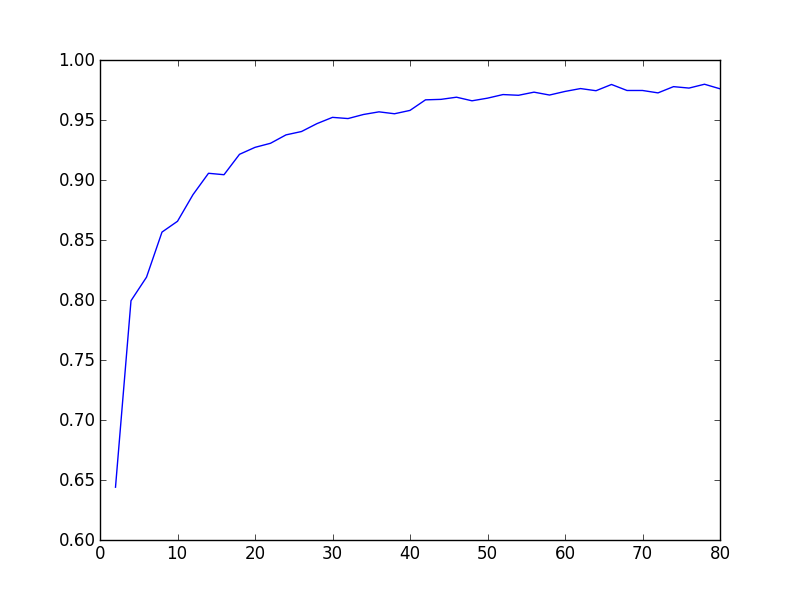
\includegraphics[scale=0.43]{test.png}
\caption{Simulated probability of recovering file as a function of the number of nodes: 10 parts, 20 codes, 66\% uptime}
\end{figure}
\begin{figure}
\centering
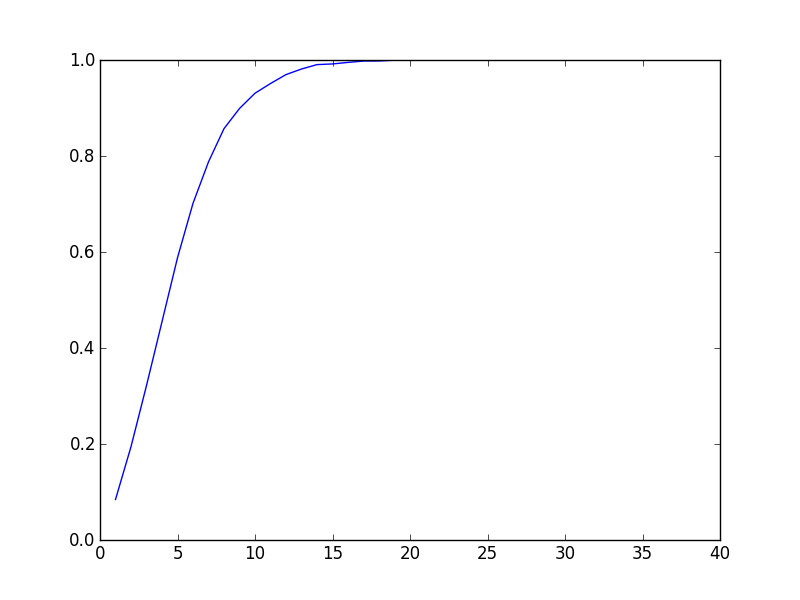
\includegraphics[scale=0.43]{test2.png}
\caption{Simulated probability of recovering file as a function of the number of codes: 10 parts, 66\% uptime, 100 nodes}
\end{figure}

\subsection{Pipeline}

Several pipelines are possible for this system. The elements of the pipeline would be compression, erasure coding and encryption. Clearly encryption cannot take place before compression because encrypted data almost never compresses at all. It is possible to compress Cauchy Reed-Solomon codes to some extent if they weren't created from encrypted data, but experiments we made show that they compress significantly less well than the original file, so clearly compression should be the first step. There is no significant difference between encrypting after creating erasure codes or before that, apart from the fact that the total amount of data to encrypt will be significantly higher if erasure coding is done first. This leads us to our final pipeline (shown in Figure 1): compression, then encryption, then erasure coding.

\begin{figure}
\centering
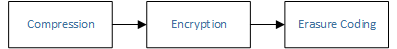
\includegraphics[scale=0.8]{flow1.png}
\caption{Our chosen pipeline}
\end{figure}

\section{Threat Model}

A major issue in a decentralized system like this one is that of security. Here we consider the security of our design against three types of attackers.

\subsection{Eavesdroppers}

Eavesdroppers want to access user data, i.e. steal user files, steal user accounts, get some knowledge of exactly what files a given user has etc.

We simply use the typical way to protect oneself against eavesdropper: cryptography is used extensively in the system. User are each assigned a RSA private key which identifies them. The vast majority of operations require a signature from the user. Users also have a single AES256 key which is stored in the distributed hash table, encrypted using the user's public key (this is because AES cryptography is much faster than RSA). All files are encrypted using this AES key and a separate random IV. Some private user data is stored that way as well. Note that a separate key could also be used for each file, though this would incur a slight performance penalty.

Because we want to provide the abstraction of a user account rather than require users to transfer their private keys across their devices, private keys are actually store in the DHT, encrypted using an AES256 key that is derived from the user "password" using PBKDF2\cite{PBKDF2} (note: a better alternative for a production system could be scrypt\cite{scrypt}, but PBKDF2 implementations are more widely available). This clearly makes the system vulnerable to dictionary attacks on passwords, so a real system should probably have a password strength verification module and should educate users about the importance of a strong password, especially in this context.

Note that an alternative would have been to generate the private key directly from the password using PBKDF2, but that would have made it extremely hard for users to change their passwords later.

Additionally, the DHT we chose to use uses public key cryptography to ensure that, for instance, nodes which do not have a user's private key are unable to delete or modify values that have been set by that user. 

\subsection{Cheaters}

Cheaters are economically motivated attackers.

An important concern in such a system as ours is the possibility of having users that use the file synchronization service without actually sharing the right amount of space to the network. The two main ways to do this would be to only connect to the network to perform actions such as storing and downloading files, or simply not actually storing the file blocks one is in charge of. 

\subsubsection{Karma}

Misbehaving nodes accumulate karma. When a node finds another node is misbehaving, it adds a karma record to the node's public karma set. Karma records exist for a limited amount of time (30 days in our current implementation) and contribute to diminishing the node's contribution to the user's overall allowed amount of storage.

For instance, if a node is found not to be connected at a given time, a NotConnected karma record will be added to it. These NotConnected records are then used to estimate the uptime of the node during the last 30 days, and the node's contribution to the overall allowed storage space for the user will be proportional its uptime. 

As another example, if a node is found to be connected but fails to prove that it does indeed store a good version of a given file part, a DeletedPart karma record will be associated with it. While it is normal for a node to be disconnected at some point, deleting a file part is considered explicitly malicious behavior and is thus harshly punished. In our implementation, three DeletedPart records within a month bring the user's allowed storage space down to 0. Unlike with disconnected nodes, the specifics of the punishment don't matter too much here, as long as they create a strong incentive to keep the file blocks.

An issue with this system is that these errors are ordinarily detected only when a client tries to download a file, which is a fairly uncommon event. For this reason, every online client will regularly keep a check on their file blocks by doing the following: when a file is added, the client generate hashes for each file block using different random salts. Then the client will regularly require nodes that store blocks from its files to compute the hash of one of their blocks using a salt they have never seen before. If the node computes a correct hash, it can be assumed that it still has the file block. If the client runs out of precached hash challenges it can always recreate a few from the files it still has locally.

\subsection{Byzantine Attackers}

Byzantine attackers could exploit issues with the system for no apparent reason. One such issue is the Sybil attack\cite{sybil}, but it is definitely out of the scope of this project. 

Another thing a Byzatine attacker might do is trying to delete data from the DHT. Fortunately, Maidsafe-DHT will allow such operations to be performed only by nodes which have the same private key as the node which initially set the value in the DHT, so this would be impossible.

Yet another is to add karma records to other nodes to reduce their maximum storage space. Unfortunately we haven't found a way to prevent this issue that would still make it possible to catch misbehaving nodes and that would be efficient, since any such method would require the help of a third party.

\section{Future Features}

\subsection{Duplicate Merging}

\subsection{File Sharing}

\subsection{Tests}

\section{Conclusions}
This paragraph will end the body of this sample document.
Remember that you might still have Acknowledgments or
Appendices; brief samples of these
follow.  There is still the Bibliography to deal with; and
we will make a disclaimer about that here: with the exception
of the reference to the \LaTeX\ book, the citations in
this paper are to articles which have nothing to
do with the present subject and are used as
examples only.
%\end{document}  % This is where a 'short' article might terminate

%ACKNOWLEDGMENTS are optional
\section{Acknowledgments}
This section is optional; it is a location for you
to acknowledge grants, funding, editing assistance and
what have you.  In the present case, for example, the
authors would like to thank Gerald Murray of ACM for
his help in codifying this \textit{Author's Guide}
and the \textbf{.cls} and \textbf{.tex} files that it describes.


\begin{thebibliography}{1}
\bibitem{dropbox} \url{http://dropbox.com}
\bibitem{drive} \url{http://drive.google.com}
\bibitem{skydrive} \url{http://skydrive.live.com}
\bibitem{icloud} \url{http://icloud.com}
\bibitem{wuala:measurement} Mager, Biersack, Michiardi, \emph{A measurement study of the {W}uala on-line storage service}, 2012
\bibitem{sync} \url{http://labs.bittorrent.com/experiments/sync.html}
\bibitem{spacemonkey} \url{http://spacemonkey.com}
\bibitem{maidsafe_site} \url{http://maidsafe.net}
\bibitem{maidsafe_dht} \url{https://code.google.com/p/maidsafe-dht/}
\bibitem{drobpox_slides} Houston, \emph{Dropbox startup lessons learned 2011}, 2011
\bibitem{compression_comparison} \url{http://bashitout.com/2009/08/30/Linux-Compression-Comparison-GZIP-vs-BZIP2-vs-LZMA-vs-ZIP-vs-Compress.html}
\bibitem{comparison_reed_solomon} Plank, \emph{A Performance Evaluation and Examination of Open-Source Erasure Coding Libraries For Storage}, 2009
\bibitem{PBKDF2} IETF, \emph{PKCS \#5: Password-Based Key Derivation Function 2 (PBKDF2) Test Vectors}, 2011
\bibitem{scrypt} Percival, \emph{Stronger Key Derivation via Sequential Memory-Hard Functions}, 2009
\end{thebibliography}


% that's all folks
\end{document}


